\documentclass[12pt]{td}
\usepackage{multicol}

\renewcommand{\TDmodule}{IUT de Montpellier, Dép. Informatique\\
M2103 - Base de la POO (1ère année)}
\renewcommand{\TDresponsables}{Responsable~: P.~Valicov}

\definecolor{commentscolor}{HTML}{568262}
\definecolor{keywordcolor}{HTML}{741157}
\definecolor{stringcolor}{HTML}{8C1C16}
\definecolor{terminaltext}{gray}{0.9}
\definecolor{terminalbg}{gray}{0.0}

\lstset{
	basicstyle=\normalsize\ttfamily\NoAutoSpacing,
	language=Java,
	commentstyle=\color{commentscolor},
	keywordstyle=\bfseries\color{keywordcolor},
	stringstyle=\color{stringcolor},
	breaklines=true,
	breakatwhitespace=true,
	keepspaces,
	columns=fullflexible,
	% literate=
	% {?}{?}1 {é}{{\'{e}}}1 {è}{{\`{e}}}1 {ê}{{\^{e}}}1 {ë}{{\¨{e}}}1 {û}{{\^{u}}}1 {ù}{{\`{u}}}1 {â}{{\^{a}}}1 {à}{{\`{a}}}1 {î}{{\^{i}}}1 {ô}{{\^{o}}}1 {ç}{{\c{c}}}1 {Ç}{{\c{C}}}1 {É}{{\'{E}}}1 {Ê}{{\^{E}}}1 {À}{{\`{A}}}1 {Â}{{\^{A}}}1 {Î}{{\^{I}}}1
}

\lstdefinestyle{terminal}{
	basicstyle=\color{terminaltext}\small\ttfamily\NoAutoSpacing,
	backgroundcolor=\color{terminalbg},
	identifierstyle=,
	commentstyle=,
	stringstyle=,
	showspaces=false,
	showstringspaces=false,
	columns=fullflexible,
	tabsize=2,
	frame=single,
	breaklines=true,
	breakatwhitespace=true,
	keepspaces,
}

\begin{document}
\title{Projet}

\newcommand{\coins}[1]{\hspace{-.2em}\makebox[1.4em]{\raisebox{-.35em}{
\includegraphics[width=1.4em]{coin.png}}\hspace{-.95em}#1\ }}
\newcommand{\vp}{\raisebox{-.4em}{
\includegraphics[height=1.4em]{vp.png}}}

\noindent
\includegraphics[width=\textwidth]{title.png}

Le but de ce projet est de produire une implémentation en \emph{Java} du jeu de cartes \emph{Dominion}.

\section{Présentation du jeu}

\emph{Dominion} est un jeu de cartes inventé par Donald X. Vaccarino pour 2 à 4 joueurs. C'est un jeu de \emph{construction de deck} où les joueurs doivent à tour de rôle jouer des cartes de leur main pour obtenir de nouvelles cartes parmi un ensemble commun disponible. Lorsque la partie s'arrête le joueur possédant le plus de points de victoire dans son deck est déclaré vainqueur.

Vous pouvez consulter les règles du jeu dans le fichier «~\texttt{Dominion-Regles.pdf}~» disponible sur l'ENT (ainsi qu'une version en anglais «~\texttt{Dominion-Rules.pdf}~»).

\bigskip
{\color{red}
\textbf{Vous êtes encouragés à lire ces règles avant de poursuivre la lecture du sujet.}
}

\bigskip
\rmq Il existe de nombreuses extensions pour \emph{Dominion} qui modifient considérablement les règles de base. Dans ce projet nous ne considérerons que le jeu de base.

\section{Les cartes}

Toutes les cartes du jeu (cf. section~\ref{sec:liste_cartes} pour la liste complète) sont caractérisées par
\begin{itemize}
	\item un nom (en haut)~;
	\item un prix d'achat (en bas à gauche)~;
	\item un type (en bas) qui peut être \emph{Trésor}, \emph{Victoire}, \emph{Malédiction}, \emph{Action}, \emph{Action/Attaque} ou \emph{Action/Réaction}~;
	\item une description (centre) qui correspond à l'effet de la carte lorsqu'elle est jouée (\emph{Action} ou \emph{Trésor}) ou comptabilisée en fin de partie (\emph{Victoire}).
\end{itemize}

Il peut exister plusieurs copies de chaque carte mais deux cartes ayant le même nom ont des caractéristiques identiques (on dira que deux cartes identiques sont de la même \emph{famille}).

Par ailleurs, l'ensemble des cartes utilisées est déterminé en début de partie et à tout moment de la partie chaque carte est
\begin{itemize}
	\item soit dans la \emph{réserve} (\emph{supply}), commune à tous les joueurs et disponible à l'achat~;
	\item soit dans la pile de cartes \emph{écartées} (\emph{trash})~;
	\item soit en la possession d'un joueur.
\end{itemize}

\subsection{La classe \texttt{Card} et ses sous-classes}

Les cartes du jeu sont représentées par des objets de la classe \texttt{Card}. Chaque carte utilisée par la partie est représentée par une instance différente, et toutes les instances sont créées au démarrage de la partie (celles qui sont initialement distribuées aux joueurs peuvent éventuellement être instanciées à la création des instances représentant les joueurs).

Étant donné que le \emph{type} d'une carte influe fortement sur la façon d'utiliser la carte, on définit une sous-classe de \texttt{Card} pour chacun des types possibles (cf. figure~\ref{fig:card_diagram})~:
\begin{description}
	\item[\texttt{TreasureCard}] pour les cartes \emph{Trésor}~;
	\item[\texttt{VictoryCard}] pour les cartes \emph{Victoire}~;
	\item[\texttt{CurseCard}] pour les cartes \emph{Malédiction}~;
	\item[\texttt{ActionCard}] pour représenter les cartes \emph{Action}.
\end{description}

Les types composés \emph{Action/Attaque} et \emph{Action/Réaction} sont représentés par deux sous-classes de \texttt{ActionCard}~: \texttt{AttackCard} et \texttt{ReactionCard} respectivement.

\begin{figure}[htbp]
	\label{fig:card_diagram}
	\begin{center}
		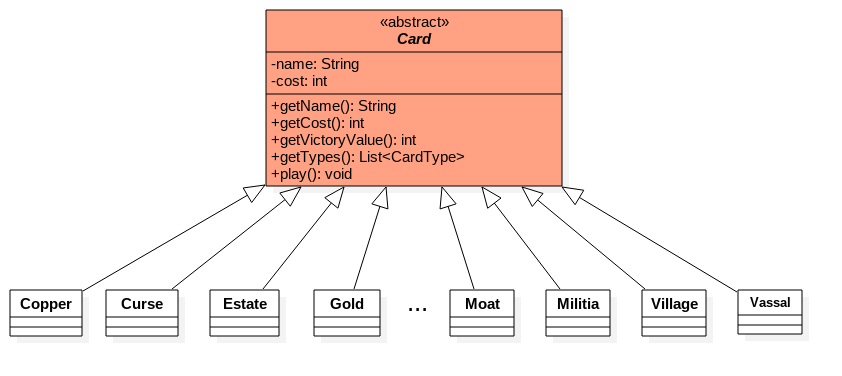
\includegraphics[width=12cm]{cardsClassDiagram.png}
	\end{center}
	\caption{Diagramme de classes de la hiérarchie représentant les cartes (pour alléger le diagramme, une seule carte est représentée pour chaque type).}
\end{figure}

\subsection{Les listes de cartes}

Afin de simplifier les tâches couramment effectuées par le jeu sur des ensembles de cartes, on définit une classe spécifique \texttt{ListOfCards} pour représenter les listes de cartes. C'est cette classe qui est utilisée pour représenter toutes les listes de cartes en possession des joueurs (main, défausse, etc.) ainsi que les piles de la réserve et la pile de cartes écartées.

Cette classe hérite de \texttt{ArrayList<Card>} ce qui permet de l'utiliser comme un \texttt{ArrayList} (constructeurs, accesseurs, méthodes) et d'ajouter des méthodes lorsque c'est utile.

La classe \texttt{ListOfCards} est fournie avec un certain nombre de méthodes supplémentaires déjà implémentées mais vous pouvez éventuellement ajouter des méthodes si vous le jugez nécessaire.

\subsection{Les types de cartes}

Pour représenter correctement les différents types possibles des cartes, un type énuméré \texttt{CardType} est fourni contenant les constantes
\begin{itemize}
	\item \texttt{Treasure}
	\item \texttt{Action}
	\item \texttt{Victory}
	\item \texttt{Curse}
	\item \texttt{Reaction}
	\item \texttt{Attack}
\end{itemize}

C'est un \texttt{ArrayList} d'éléments de ce type qui est renvoyé par la méthode \texttt{getTypes()} de la classe \texttt{Card} (les cartes du jeu de base peuvent avoir un ou deux types).

%%%%%%%%%%%%%%%%%%%%%%%%%%%%%%%%%%%%%%%%%%%%%%%%%%%%%%%%%%%%%%%%%%%%%%%%%%%%%%%%

\section{Les joueurs}

Les joueurs de la partie sont identifiés par un nom (de type \texttt{String}). À tout moment de la partie, les cartes que possède un joueur peuvent être dans l'un des 4 emplacements suivants~:
\begin{itemize}
	\item sa \emph{main} (\emph{hand})~;
	\item sa \emph{défausse} (\emph{discard})~;
	\item sa \emph{pioche} (\emph{draw})~;
	\item la liste des cartes actuellement \emph{en jeu} (\emph{in play}).
\end{itemize}

L'ensemble des cartes possédées par le joueur (dans l'un des emplacements précédemment cités) constitue le \emph{deck} du joueur. Chaque joueur commence la partie avec 3 cartes \emph{Estate} et 7 cartes \emph{Copper} dans sa défausse (et en pioche immédiatement 5 en main).

En plus de ses cartes, un joueur a différents compteurs de ressources~:
\begin{itemize}
	\item le nombre d'\emph{actions} qu'il peut jouer (initialisé à 1 au début de son tour)~;
	\item le nombre de pièces dont il dispose pour acheter des cartes (initialisé à 0 au début de son tour)~;
	\item le nombre d'achats qu'il peut réaliser (initialisé à 1 au début de son tour)
\end{itemize}

\subsection{Déroulement du tour}

Le tour d'un joueur s'exécute en plusieurs étapes
\begin{description}
	\item[Préparation.] Les compteurs du joueur sont remis aux valeurs indiquées par les règles~: 1 pour les actions et les achats, et 0 pour l'argent.
	\item[Actions.] Le joueur peut jouer des cartes \emph{Action} de sa main tant que son compteur d'actions est supérieur ou égal à 1. Lorsqu'une carte \emph{Action} est jouée, le compteur d'actions du joueur est décrémenté de 1, la carte jouée est marquée comme étant \emph{en jeu} et l'action de la carte est exécutée. Le joueur peut choisir de passer à la phase suivante même s'il lui reste des actions qu'il peut jouer.
	\item[Trésors.] Le joueur peut jouer des cartes \emph{Trésor} de sa main. Dans le jeu de base, il n'y a aucune situation ou le joueur aurait un intérêt à conserver des trésors dans sa main. On pourra donc considérer ici que le joueur joue automatiquement tous les trésors qu'il a en main.
	\item[Achats.] Le joueur peut acheter des cartes de la réserve en utilisant l'argent qu'il a amassé pendant les phases précédentes. Le joueur peut acheter une carte s'il lui reste au moins un achat et que le prix de la carte est inférieur à la somme dont il dispose. Lorsqu'il achète une carte, son compteur d'achats est décrémenté de 1, son argent de la valeur de la carte achetée et la carte achetée est déplacée dans la défausse du joueur. Le joueur peut choisir de terminer cette phase même s'il peut encore acheter des cartes.
	\item[Fin.] À la fin du tour toutes les cartes de la main du joueur et en jeu sont défaussées, les compteurs du joueur sont remis à 0 et le joueur pioche 5 nouvelles cartes en main.
\end{description}
	\rmq Il est important que les cartes en main soient piochées à la fin du tour car la main peut être affectée pendant le tour d'un autre joueur (cf. \emph{Militia} ou \emph{Moat} par exemple).

\subsection{La classe \texttt{Player}}

Les joueurs participant à une partie de \emph{Dominion} sont représentés par des instances d'une classe \texttt{Player}. Le nom, les compteurs (actions, argent, achats), les différentes piles de cartes du joueur ainsi que la partie dans laquelle il se trouve sont représentés par des attributs.

La figure~\ref{fig:game_diagram} illustre les attributs et méthodes qui doivent être implémentés dans la classe \texttt{Player} (voir le code fourni pour les spécifications de chaque méthode). Vous pouvez cependant ajouter des méthodes si vous le jugez nécessaire.

\begin{figure}[htbp]
	\centering
		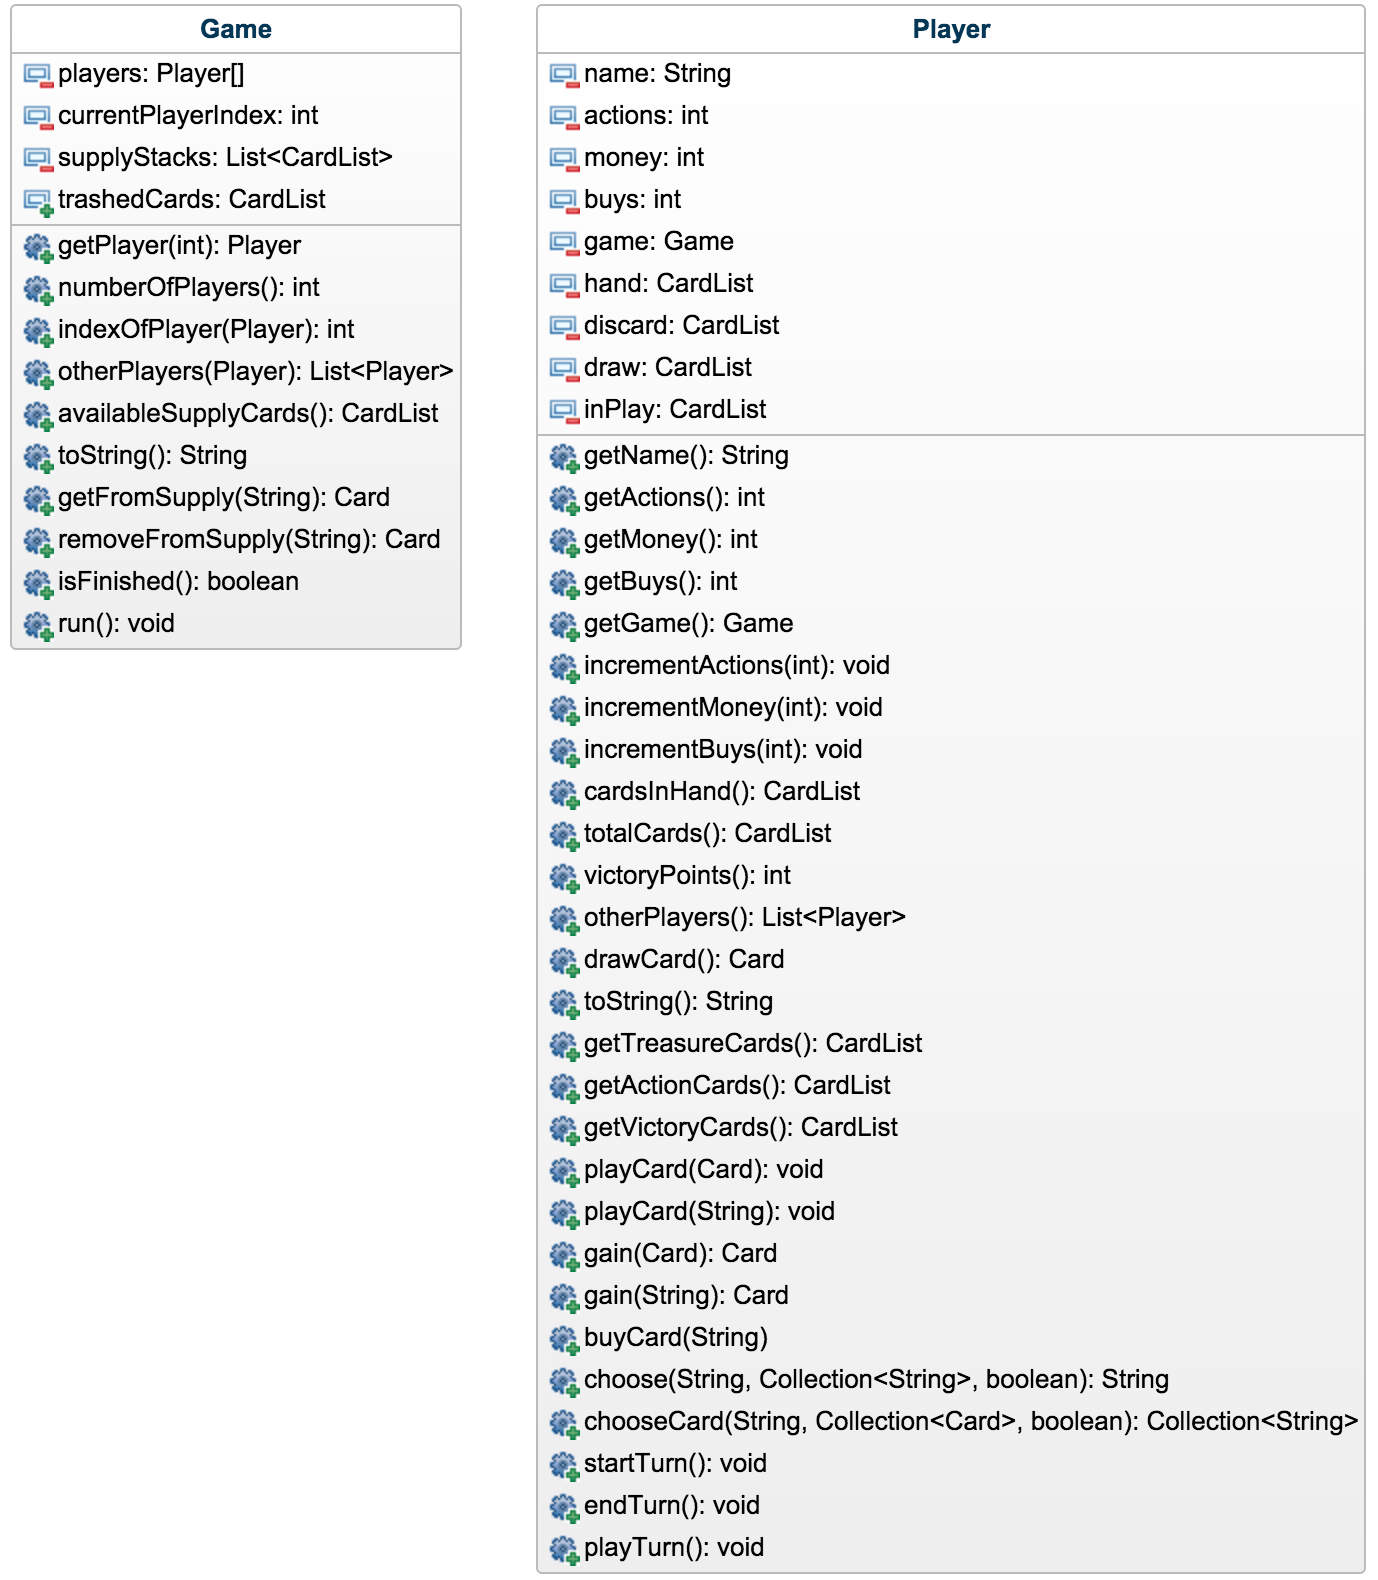
\includegraphics[width=12cm]{game_diagram.png}
	\caption{Diagramme des classes \texttt{Game} et \texttt{Player}.}
	\label{fig:game_diagram}
\end{figure}


%%%%%%%%%%%%%%%%%%%%%%%%%%%%%%%%%%%%%%%%%%%%%%%%%%%%%%%%%%%%%%%%%%%%%%%%%%%%%%%%

\section{La partie}

Une partie de \emph{Dominion} est représentée par une instance de la classe \texttt{Game}. C'est la partie qui gère la liste des joueurs, l'ensemble des cartes communes et qui contrôle le déroulement de la partie~: mise en place, alternance des tours des joueurs et fin de partie lorsque les conditions de fin sont remplies.

Pour démarrer une partie, il faut spécifier le nombre de joueurs qui y participent ainsi que la liste des cartes à utiliser comme piles de réserve. Le constructeur de la classe \texttt{Game} prend donc deux arguments~:
\begin{description}
	\item[\texttt{String[] playerNames} :] la liste des noms des joueurs qui participent à la partie (c'est le constructeur de \texttt{Game} qui construit les instances de \texttt{Player} correspondantes)
	\item[\texttt{List<ListOfCards> kingdomPiles} :] une liste de piles de réserve à utiliser comme cartes \emph{Royaume} dans la partie. Les règles du jeu prévoient 10 piles \emph{Royaume} mais la partie peut fonctionner avec un nombre différent. Le constructeur de \texttt{Game} doit ajouter à ces piles les piles de réserve communes (cartes \emph{Trésor}, \emph{Victoire} et \emph{Malédiction})
\end{description}

La classe \texttt{Game} est relativement simple (par rapport à \texttt{Player}), et la figure~\ref{fig:game_diagram} illustre les attributs et méthodes qu'il vous est demandé d'écrire. Comme précédemment, vous pouvez ajouter des méthodes si cela vous semble nécessaire.

%%%%%%%%%%%%%%%%%%%%%%%%%%%%%%%%%%%%%%%%%%%%%%%%%%%%%%%%%%%%%%%%%%%%%%%%%%%%%%%%

\section{Interface utilisateur}

Pour des raisons de simplicité, seule une interface en ligne de commande vous est demandée. Une fois la partie lancée, toutes les interactions avec l'utilisateur se feront donc dans le terminal. Les informations du jeu seront affichées à l'écran en utilisant la sortie standard et les choix des joueurs se feront par lecture sur l'entrée standard (clavier).

Dans une partie à plusieurs joueurs, un même processus demande successivement aux joueurs de jouer leur tour dans le même terminal.

\subsection{Choix}

Lorsqu'un joueur doit choisir parmi un ensemble de cartes (par exemple la carte à jouer dans sa main, ou une carte à acheter dans la réserve ou encore une carte parmi deux \emph{Trésors} après avoir joué un \emph{Voleur}), il devra entrer le nom exact de la carte choisie (on utilisera les noms anglais des cartes pour éviter les problèmes de caractères accentués). Par exemple, il pourra choisir \texttt{"Village"} ou \texttt{"Throne Room"}.

Pour indiquer qu'il souhaite \emph{passer} (par exemple parce qu'il ne souhaite pas jouer de carte \emph{Action}, qu'il ne veut rien acheter en fin de tour ou encore s'il ne veut plus écarter de cartes après avoir joué une \emph{Chapelle}), le joueur entrera la chaîne de caractères vide \texttt{""}.

Enfin, lorsqu'il doit faire un choix parmi deux possibilités (par exemple choisir s'il veut défausser son deck après avoir joué un \emph{Chancellier}, ou s'il veut défausser une carte \emph{Action} piochée après avoir joué une \emph{Biliothèque}), il répondra à une question posée en entrant \texttt{"y"} pour oui et \texttt{"n"} pour non.

%%%%%%%%%%%%%%%%%%%%%%%%%%%%%%%%%%%%%%%%%%%%%%%%%%%%%%%%%%%%%%%%%%%%%%%%%%%%%%%%

\section{Rendu attendu}

Vous devez fournir une archive au format \texttt{zip} ou \texttt{tar} contenant les fichiers \texttt{.java} complétés. Cette archive doit respecter exactement la hiérarchie de répertoires et les noms de fichiers du code qui vous a été fourni (vous devriez simplement compléter les fichiers fournis).

Toutes les méthodes indiquées dans le code fourni doivent être complétées selon les spécifications (en respectant les noms et les paramètres indiqués). Vous pouvez éventuellement ajouter des attributs et méthodes aux classes, lorsque cela vous semble nécessaire.

L'exécution de la méthode \texttt{main} de la classe \texttt{Main} (à la racine du projet) doit démarrer une partie avec un ensemble de 10 cartes \emph{Royaume} de votre choix (cette fonction servira simplement à tester manuellement la bonne exécution d'une partie, mais l'ensemble des cartes sera évalué par la suite de manière automatique, indépendamment du choix de cartes pour la partie exécutée par la méthode \texttt{main}).

\subsection{Évaluation}

L'évaluation du projet se fera à l'aide de tests automatisés. Un premier jeu de tests vous sera fourni avant la fin du projet pour que vous puissiez vérifier le bon fonctionnement des fonctionnalités de base, puis nous utiliserons un second jeu de tests (secret) pour l'évaluation finale.

Il est donc attendu que les projets rendus passent le premier jeu de tests sans erreurs, mais vous devez également vérifier par vous-mêmes que le projet se comporte correctement dans les différents cas particuliers qui peuvent se produire et qui ne sont pas nécessairement couverts par ces premiers tests.

%%%%%%%%%%%%%%%%%%%%%%%%%%%%%%%%%%%%%%%%%%%%%%%%%%%%%%%%%%%%%%%%%%%%%%%%%%%%%%%%

\newpage
\section{Liste des cartes}
\label{sec:liste_cartes}

\newcommand{\card}[3]{
	\noindent
	\begin{minipage}{.15\textwidth}
	\includegraphics[width=\textwidth]{cards/#1.jpg}
	\end{minipage}
	\begin{minipage}{.35\textwidth}
	\textbf{\emph{#2}}\\
	#3
	\end{minipage}
}

\subsection{Cartes communes}

\begin{multicols}{2}
	\card{copper}{Cuivre (Copper)}{+\coins{1}}
	\card{silver}{Argent (Silver)}{+\coins{2}}
\end{multicols}
\begin{multicols}{2}
	\card{gold}{Or (Gold)}{+\coins{3}}
\end{multicols}
\begin{multicols}{2}
	\card{estate}{Domaine (Estate)}{1\vp}
	\card{duchy}{Duché (Duchy)}{3\vp}
\end{multicols}
\begin{multicols}{2}
	\card{province}{Province}{6\vp}
\end{multicols}
\begin{multicols}{2}
	\card{curse}{Malédiction (Curse)}{-1\vp}
\end{multicols}


%%%%%%%%%%%%%%%%%%%%%%%%%%%%%%%%%%%%%%%%%%%%%%%%%%%%%%%%%%%%%%%%%%%%%%%%%%%%%%%%

\renewcommand{\card}[4]{
	\bigskip

	\noindent
	\begin{minipage}{.15\textwidth}
	\includegraphics[width=\textwidth]{cards/#1.jpg}
	\end{minipage}
	\begin{minipage}{.85\textwidth}
	\textbf{\emph{#2}}\\
	#3
	\bigskip\\
	\textbf{Détails~: }#4
	\end{minipage}
} 
\newcommand{\details}{\textbf{Détails~: }}

\newpage
\subsection{Cartes royaume}

\card{cellar}{Cave (Cellar)}{+1 Action.\\Défaussez autant de cartes que vous voulez.\\+1 Carte par carte défaussée.}
{Le joueur entre un par un les noms des cartes qu'il souhaite défausser de sa main. Lorsqu'il ne veut plus défausser de cartes, il entre la chaîne vide. Le programme doit compter les cartes défaussées et ne piocher les nouvelles cartes en main qu'après que l'utilisateur ait fini de défausser.}

\card{chapel}{Chapelle (Chapel)}{Écartez jusqu'à 4 cartes de votre main.}
{Le joueur entre un par un les noms des cartes à écarter. Il peut entrer la chaîne vide lorsqu'il ne souhaite plus écarter de carte.}

\card{moat}{Douves (Moat)}{+2 Cartes.\\Lorsqu'un adversaire joue une carte \emph{Attaque}, vous pouvez dévoiler cette carte de votre main.\\Dans ce cas, l'\emph{Attaque} n'a pas d'effet sur vous.}
{La carte est très simple lorsqu'elle est jouée en tant que carte \emph{Action}. C'est en tant que réaction à une attaque qu'elle est plus complexe. Lorsqu'un joueur joue une carte \emph{Attaque}, il faut demander à tous les autres joueurs ayant des \emph{Douves} en main s'ils veulent la révéler. S'ils répondent \texttt{"y"}, alors l'attaque ne les affecte pas, s'ils répondent \texttt{"n"} ils subissent l'attaque normalement (comme s'ils n'avaient pas de \emph{Douves} en main).}

\card{chancellor}{Chancellier (Chancellor)}{+\coins{2}.\\Vous pouvez immédiatement défausser votre deck.}
{Le programme demande au joueur s'il veut défausser son deck. S'il répond \texttt{"y"} le deck est placé dans la défausse. S'il répond \texttt{"n"} aucun effet supplémentaire ne se produit.}

\card{village}{Village}{+1 Carte.\\+2 Actions.}
{Aucune intervention de la part des joueurs.}

\card{woodcutter}{Bûcheron (Woodcutter)}{+1 Achat.\\+\coins{2}.}
{Aucune intervention de la part des joueurs.}

\card{workshop}{Atelier (Workshop)}{Recevez une carte coûtant jusqu'à \coins{4}.}
{Le joueur doit entrer le nom de la carte qu'il souhaite gagner.}

\card{bureaucrat}{Bureaucrate (Bureaucrat)}{Recevez une carte \emph{Argent}~; placez-la sur votre deck.\\Tous vos adversaires dévoilent une carte \emph{Victoire} et la placent sur leur deck (sinon ils dévoilent leur main afin que vous puissiez voir qu'ils n'ont pas de cartes \emph{Victoire}).}
{Les adversaires doivent entrer le nom de la carte \emph{Victoire} qu'ils souhaitent révéler (s'ils n'en ont aucune, le programme passe automatiquement au joueur suivant).}

\card{feast}{Festin (Feast)}{Écartez cette carte.\\Recevez une carte coûtant jusqu'à \coins{5}.}
{La carte est automatiquement écartée. Le joueur doit indiquer le nom de la carte qu'il souhaite gagner.}

\card{gardens}{Jardins (Gardens)}{Vaut 1\vp{} pour chaque 10 cartes dans votre deck (arrondi à l'unité inférieure).}
{Pour obtenir la valeur de cette carte, il faut compter toutes les cartes en possession du joueur (main, défausse, pioche et en jeu). Si la carte dit qu'il faut compter les cartes dans le \emph{deck} (terme qui est habituellement utilisé pour la pioche dans le reste des règles) c'est parce que d'après les règles en fin de partie toutes les cartes du joueur sont placées dans sa pioche (donc son \emph{deck}) avant de compter les points. Pour le programme, il est plus simple de compter les cartes dans toutes les piles appartenant au joueur.}

\card{militia}{Milice (Militia)}{+\coins{2}.\\Tous vos adversaires défaussent leurs cartes de façon à n'avoir que 3 cartes en main.}
{Chaque adversaire doit entrer les noms des cartes qu'il souhaite défausser de sa main, tant qu'il a strictement plus de 3 cartes.}

\card{moneylender}{Prêteur sur gages (Moneylender)}{Écartez une carte \emph{Cuivre} de votre main.\\Dans ce cas, +\coins{3}.}
{Aucune intervention de la part des joueurs. Écarter un cuivre n'est pas optionnel (si le joueur en a un) et peut donc être fait automatiquement par le programme.}

\card{remodel}{Rénovation (Remodel)}{Écartez une carte de votre main.\\Recevez une carte coûtant jusqu'à \coins{2} de plus que la carte écartée.}
{Le joueur entre le nom de la carte de sa main qu'il souhaite écarter, puis le nom de la carte qu'il souhaite gagner.}

\card{smithy}{Forgeron (Smithy)}{+3 Cartes.}
{Aucune intervention de la part des joueurs.}

\card{spy}{Espion (Spy)}{+1 Carte.\\+1 Action.\\Tous les joueurs (vous aussi) dévoilent la première carte de leur deck. Vous décidez ensuite si chaque carte dévoilée est défaussée ou replacée sur son deck.}
{Pour chaque carte dévoilée (en commençant par le joueur qui a joué l'\emph{Espion} et en suivant dans le sens du jeu) le joueur doit entrer \texttt{"y"} s'il souhaite défausser la carte dévoilée, et \texttt{"n"} s'il souhaite qu'elle soit replacée sur le deck.}

\card{thief}{Voleur (Thief)}{Tous vos adversaires dévoilent les 2 premières cartes de leur deck. S'ils dévoilent des cartes \emph{Trésor}, ils en écartent 1 de votre choix. Parmi ces cartes \emph{Trésor} écartées, recevez celles de votre choix. Les autres cartes dévoilées sont défaussées.}
{Chaque adversaire révèle 2 cartes, puis le joueur qui a joué le \emph{Voleur} doit entrer le nom de la carte qu'il souhaite écarter (seulement s'il y a deux Trésors distincts révélés, mais dans les autres cas la fonction \texttt{chooseCard} peut automatiquement faire le choix). Lorsque toutes les cartes des adversaires ont été écartées, le joueur peut choisir de gagner certaines des cartes écartées (ce choix se fait à la fin, pas après chaque carte écartée). Il entre alors les noms des cartes qu'il souhaite gagner, et peut entrer la chaîne vide lorsqu'il ne souhaite plus gagner de cartes.}

\card{throneroom}{Salle du trône (Throne Room)}{Choisissez 1 carte \emph{Action} de votre main.\\Jouez-la deux fois.}
{Le joueur entre le nom de la carte \emph{Action} de sa main qu'il souhaite jouer deux fois. L'action de la carte est exécutée deux fois par le programme (avec toutes les interactions associées). Notez que le joueur peut tout à fait jouer une seconde \emph{Salle du trône} deux fois, mais il faut alors qu'il ait deux autres actions en main, puisque chaque exécution de la seconde \emph{Salle du trône} demande que le joueur ait une carte en main (lorsqu'une carte est jouée avec \emph{Salle du trône} elle est mise en jeu).}

\card{councilroom}{Chambre du conseil (Council Room)}{+4 Cartes.\\+1 Achat.\\Tous vos adversaires piochent 1 carte.}
{Aucune intervention de la part des joueurs.}

\card{festival}{Festival}{+2 Actions.\\+1 Achat.\\+\coins{2}.}
{Aucune intervention de la part des joueurs.}

\card{laboratory}{Laboratoire (Laboratory)}{+2 Cartes.\\+1 Action.}
{Aucune intervention de la part des joueurs.}

\card{library}{Bibliothèque (Library)}{Piochez jusqu'à ce que vous ayez 7 cartes en main. Chaque carte \emph{Action} piochée peut être mise de côté. Défaussez les cartes mises de côté lorsque vous avez terminé de piocher.}
{Les cartes sont automatiquement piochées tant que le joueur a strictement moins de 7 cartes en main. À chaque fois qu'une carte Action est piochée, le joueur peut entrer \texttt{"y"} pour la mettre de côté (ou \texttt{"n"} pour la piocher en main normalement).}

\card{market}{Marché (Market)}{+1 Carte.\\+1 Action.\\+1 Achat.\\+\coins{1}.}
{Aucune intervention de la part des joueurs.}

\card{mine}{Mine}{Écartez une carte \emph{Trésor} de votre main. Recevez une carte \emph{Trésor} coûtant jusqu'à \coins{3} de plus~; ajoutez cette carte à votre main.}
{Le joueur doit entrer le nom de la carte qu'il souhaite écarter, puis le nom de la carte qu'il souhaite gagner.}

\card{witch}{Sorcière (Witch)}{+2 Cartes.\\Tous vos adversaires recoivent une carte \emph{Malédiction}.}
{Aucune intervention de la part des joueurs.}

\card{adventurer}{Aventurier (Adventurer)}{Dévoilez des cartes de votre deck jusqu'à ce que 2 cartes \emph{Trésor} soient dévoilées. Ajoutez ces cartes \emph{Trésor} à votre main et défaussez les autres cartes dévoilées.}
 {Aucune intervention de la part des joueurs.}

\end{document}
